\documentclass[conference,letterpaper]{IEEEtran}
\usepackage{mathptmx}
\usepackage[T1]{fontenc}
\usepackage{graphicx,amsmath,booktabs,url,tikz}
\usetikzlibrary{arrows.meta,positioning}
\title{Chip Orchestra for Observable RTL to Padframe Design}
\author{\IEEEauthorblockN{Ade Irman Budi Hendrawan, William Anthony, Rifky Afriadi, Radhian Ferel Armansyah}
\IEEEauthorblockA{School of Electrical Engineering and Informatics\\Bandung Institute of Technology (ITB)\\Bandung, Indonesia\\
\{adeirman2705, willomooi, rifki.afriyadi, radhianarmansyah\}@gmail.com}}
\begin{document}
\maketitle
\begin{abstract}
Open-source physical design flows make digital implementation accessible, but moving from generated register-transfer-level descriptions to a chip-level padframe requires coordinated verification, artifact management, and explicit acceptance criteria. We present Chip Orchestra, a browser-based platform that connects behavioral references, hierarchical hardware generation, electronic design automation tools, and a GlobalFoundries 180 nm padframe backend. The platform retains stage reports and tool logs, supports bounded repair, and requires human review of reference outputs before hardware generation. Its backend combines a hardened core with a reusable input/output ring and emits chip-level layout and handoff artifacts. We evaluate the methodology using an actor--critic maze case record, retained coarse-grained reconfigurable-array implementation reports, and a new NanoCGRA padframe assembly run. The maze case reports agreement on all 64 output cells, 13 passing checks, and 12,114 cycles. Fresh NanoCGRA RTL simulation passes static random-access memory, addition, multiplication, and exclusive-or transactions through its universal asynchronous receiver/transmitter interface. Assembly of the retained 466.555 micrometer square core produces a 2.935 mm square chip hierarchy with four signal routes and seven supply routes, visualized directly in KLayout. These geometric routes are best-effort and do not establish electrical connectivity or full-chip signoff. The results demonstrate an inspectable route from behavioral intent to physical assembly while distinguishing verified core behavior from remaining chip-level acceptance requirements.
\end{abstract}
\begin{IEEEkeywords}
RTL to padframe, chip design automation, hardware verification, open-source EDA, AI orchestration
\end{IEEEkeywords}

\section{Introduction}
Generating register-transfer-level (RTL) code is only one step in building an application-specific integrated circuit (ASIC). A useful design must satisfy a behavioral specification, survive synthesis and physical implementation, and connect to external signals and supplies through an input/output (I/O) padframe. A completed core layout does not establish that the surrounding chip is electrically connected or physically verified. This boundary becomes especially important when large language models (LLMs) generate hardware and modify implementation constraints.

OpenROAD provides an open-source foundation for digital physical implementation~\cite{openroad}. LibreLane coordinates implementation tools through a configurable flow~\cite{librelane}. These capabilities reduce dependence on proprietary infrastructure, but a project still needs a common representation of intent, verification outcomes, generated artifacts, and engineer decisions. Chip Orchestra addresses this coordination problem by treating design execution as an observable graph of stages rather than a sequence of opaque tool invocations.

The contribution is a platform integration with three concrete properties. First, executable behavioral references precede RTL generation and are exposed for human review. Second, stage reports connect generated files, verification outcomes, and bounded repair attempts to a task. Third, a dedicated padframe backend assembles the hardened core into a reusable GlobalFoundries 180 nm microcontroller (GF180MCU) ring and emits physical handoff artifacts. The work does not claim a new placement algorithm or a measured reduction in engineering effort. Its research question is whether these interfaces provide an inspectable route from design intent to chip assembly.

Section II describes the orchestration and padframe methodology. Section III presents the accelerator case studies. Section IV discusses evidence, reproducibility, and limitations. Section V concludes the paper.

\section{Orchestration and Padframe Methodology}
\subsection{Execution and Behavioral Acceptance}
The platform separates the browser interface, a Go orchestration service, a Python agent service, and a Python electronic design automation (EDA) service. MySQL stores task state and Redis supports caching and event delivery. The scheduler represents dependencies as a directed acyclic graph. Stage reports retain artifact paths, metrics, summaries, and raw log locations. Fig.~\ref{fig:flow} summarizes the logical path without assuming that every stage has passed for every design.

The golden-reference stage creates executable Python behavior, test suites, and input/expected-output vectors for design modules. A successful reference-generation stage enters an awaiting-approval state. The engineer reviews the computed output before RTL generation is released. This gate addresses specification interpretation, which a compiler or physical checker cannot assess. Subsequent self-checking testbenches compare RTL behavior with the accepted reference. A shared reference can still contain an error, so independent properties and additional workloads remain necessary.

\begin{figure}[t]
\centering
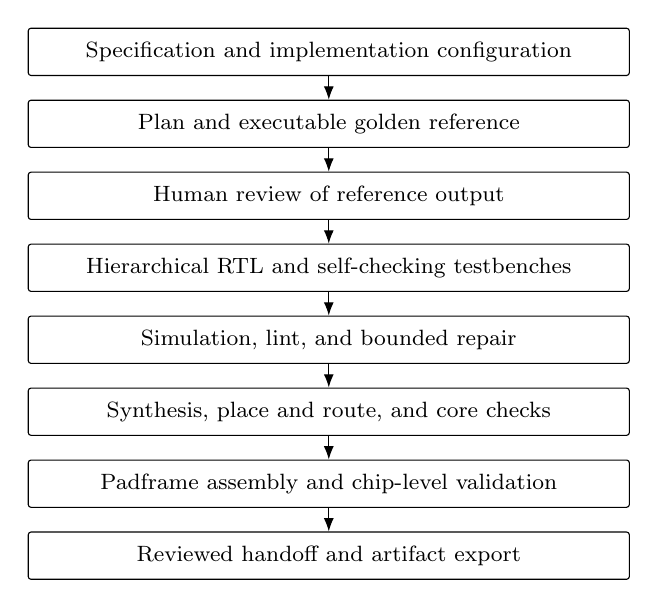
\begin{tikzpicture}[node distance=3mm,box/.style={draw,rounded corners=1pt,align=center,text width=7.4cm,minimum height=6mm,font=\footnotesize},>=Latex]
\node[box] (a) {Specification and implementation configuration};
\node[box,below=of a] (b) {Plan and executable golden reference};
\node[box,below=of b] (c) {Human review of reference output};
\node[box,below=of c] (d) {Hierarchical RTL and self-checking testbenches};
\node[box,below=of d] (e) {Simulation, lint, and bounded repair};
\node[box,below=of e] (f) {Synthesis, place and route, and core checks};
\node[box,below=of f] (g) {Padframe assembly and chip-level validation};
\node[box,below=of g] (h) {Reviewed handoff and artifact export};
\foreach \s/\t in {a/b,b/c,c/d,d/e,e/f,f/g,g/h}{\draw[->] (\s)--(\t);}
\end{tikzpicture}
\caption{Logical Chip Orchestra workflow. Stage completion, behavioral acceptance, and physical validation are distinct decisions.}
\label{fig:flow}
\end{figure}

\subsection{Core Implementation and Repair}
The EDA service invokes simulation, lint, synthesis, and physical implementation tools. Generated RTL uses a hierarchy of leaf modules, intermediate integrators, and a chip top. A corresponding testbench is produced for each module. Icarus Verilog and Verilator support functional and static checking, while Yosys and OpenROAD support technology mapping and physical implementation. GF180MCU supplies the process design kit (PDK), standard-cell views, I/O cells, and physical rules~\cite{gf180}.

Repair loops consume diagnostic results under a configured budget. A repair changes the candidate design, so acceptance must be tied to the resulting files rather than to a previous successful run. Physical timing results are interpreted with their clock period, library corner, and stage of extraction. A simulation clock is a stimulus parameter and must not be substituted for the achieved post-route frequency.

\subsection{Padframe Assembly}
The inspected backend supports the \texttt{gf180-v1} configuration. It declares a $2935\times2935\,\mu$m die, a $0.005\,\mu$m grid, and GF180MCU I/O cell classes. The declared ring contains 58 analog pads, two digital input pads for clock and reset, two bidirectional pads for universal asynchronous receiver/transmitter (UART) signals, three digital supply pads, four digital ground pads, and four corners. These are ring resources rather than 69 independently exercised user signals.

The native Python assembler uses \texttt{gdspy} to read the bundled ring and hardened-core Graphic Data System II (GDSII) files. It rejects missing files, missing top-level cells, and unavailable bounding boxes. It merges cell libraries, prefixes colliding core names, creates a chip top, and inserts references to the ring and translated core. For ring center $\mathbf{c}_r$ and core center $\mathbf{c}_c$, the translation is
\begin{equation}
\mathbf{t}=\mathbf{c}_r-\mathbf{c}_c .
\label{eq:center}
\end{equation}
Here $\mathbf{t}$ is the two-dimensional core offset. Centering provides geometric placement, but a separate fit check must establish containment inside the usable opening and any required keep-out region.

The routing routine adds signal metal on Metal2 and supply straps on Metal3. The configuration places clock and reset on the south edge and UART on the west edge, where the reusable ring provides the required bidirectional cells. It matches signal names against core DEF pins, but route endpoints use estimated pad geometry and distributed core-edge points rather than actual pin shapes. Route counts therefore establish geometric assembly, not electrical connectivity. Fig.~\ref{fig:ring} shows the arrangement schematically.

\begin{figure}[t]
\centering
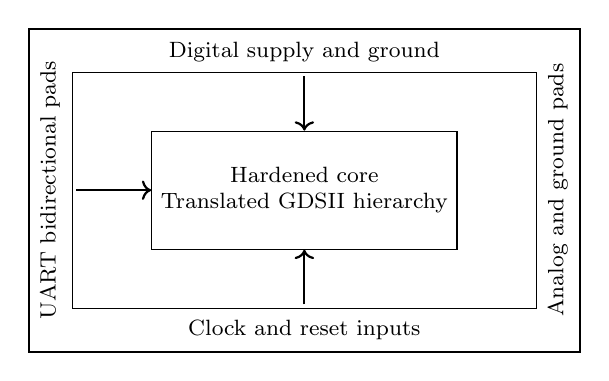
\begin{tikzpicture}[x=1cm,y=1cm,font=\footnotesize]
\draw[thick] (0,0) rectangle (7,4.1);
\draw (0.55,0.55) rectangle (6.45,3.55);
\node[draw,minimum width=3.2cm,minimum height=1.5cm,align=center] (core) at (3.5,2.05) {Hardened core\\Translated GDSII hierarchy};
\node[fill=white,align=center] at (3.5,3.8) {Digital supply and ground};
\node[fill=white,align=center] at (3.5,0.27) {Clock and reset inputs};
\node[rotate=90,fill=white] at (0.27,2.05) {UART bidirectional pads};
\node[rotate=90,fill=white] at (6.72,2.05) {Analog and ground pads};
\draw[->,thick] (0.6,2.05)--(core.west);
\draw[->,thick] (3.5,0.6)--(core.south);
\draw[->,thick] (3.5,3.5)--(core.north);
\end{tikzpicture}
\caption{Schematic of the implemented ring configuration and pad-to-core connection roles. Ring die size is 2.935 mm square.}
\label{fig:ring}
\end{figure}

The handoff set includes GDSII, a Design Exchange Format (DEF) placement, a Library Exchange Format (LEF) abstract, a Verilog ring netlist, a resolved configuration, previews, and a log. A historical external padring binary is attempted for supporting artifacts. If unavailable, deterministic supporting files can be emitted. Native binary GDSII assembly is still required. The report field \texttt{used\_real\_tools} reflects binary GDS generation and is not a design-rule or connectivity verdict.

\section{Case Studies and Results}
\subsection{Actor--Critic Maze Accelerator}
The supplied manuscript describes a Deep Deterministic Policy Gradient (DDPG) actor--critic accelerator~\cite{ddpg} with an on-chip $8\times8$ maze environment. We use this as a reported functional and core-implementation case. The provided material does not include the underlying DDPG run directory, so its numerical results are attributed to that case record rather than presented as measurements repeated in this study.

The design uses signed eight-bit weights and activations, a 22-bit multiply--accumulate accumulator, a $16\rightarrow16\rightarrow4$ actor, and a $20\rightarrow16\rightarrow1$ critic. A 64-entry replay buffer stores 276 bits per experience. A controller sequences state observation, action selection, environment updates, experience storage, and critic evaluation. The documented inference policy selects the highest action score. A discrete argmax policy and replay-buffer hardware alone do not establish implementation of the complete DDPG training algorithm, which also requires parameter updates and target-network handling.

The documented episode begins at $(1,4)$ and ends at $(7,7)$. It passes 13 self-checks and matches the reference on all 64 maze cells. Fig.~\ref{fig:maze} preserves the input and output visualization from the supplied document. The case reports a 17-step path and 12,114 execution cycles. For cycle count $N$ and clock frequency $f$, episode latency is
\begin{equation}
T_{\mathrm{episode}}=N/f .
\end{equation}
Here $T_{\mathrm{episode}}$ is elapsed execution time. The reported count corresponds to $121.14\,\mu$s at the 100 MHz simulation clock, or approximately $984.9\,\mu$s at the 12.3 MHz physical-design clock. The latter is a conversion of the cycle count, not a silicon measurement.

\begin{figure}[t]
\centering
\includegraphics[width=3.3in]{figures/image1.png}
\caption{Supplied maze case visualization. The output path is distinguishable from free cells by shading, while start and goal carry letter labels. Reported agreement is 64 of 64 cells.}
\label{fig:maze}
\end{figure}

Table~\ref{tab:ddpg} lists the principal reported core results. The $0.426$ mm$^2$ maze core-design die must not be described as the $8.614$ mm$^2$ NanoCGRA padframe die. They refer to different designs and physical boundaries. The original manuscript's internal-power estimate is omitted because its switching assumptions and power scope cannot be verified from the supplied package.

\begin{table}[t]
\caption{Reported Maze Accelerator Core Results}
\label{tab:ddpg}\centering\small
\begin{tabular}{ll}\toprule
Metric & Supplied case record\\\midrule
Reference agreement & 64/64 cells\\
Self-checks & 13/13 passing\\
Episode & 12,114 cycles, 17 steps\\
Core-design die & $643.68\times661.6\,\mu$m\\
Standard cells & 21,319\\
Core utilization & 49.08\%\\
Physical clock & 12.3 MHz\\
Setup / hold slack & $+5.05$ / $+0.42$ ns\\
DRC / LVS / antenna & Zero violations reported\\\bottomrule
\end{tabular}
\end{table}

\begin{figure}[t]
\centering
\includegraphics[width=3.1in]{figures/nanocgra_padframe_klayout.png}
\caption{KLayout screenshot of the newly assembled NanoCGRA GDSII. The 2.935 mm square ring surrounds the retained 466.555 $\mu$m square core. Visible geometric routes are not electrically signed off.}
\label{fig:padframe}
\end{figure}

\subsection{Repository-Held Reconfigurable Array}
The repository additionally contains physical implementation reports for NanoCGRA-Lite, a coarse-grained reconfigurable array (CGRA). Its optimized variant has nine processing elements, 32 bytes of static random-access memory (SRAM), and a UART bridge that replaces the parallel host interface. The retained comparison reports a reduction from 39 to four signal pins, at a synthesized-cell increase from 5,082 to 5,296. The gate area rises from 116,523 to 123,634 $\mu$m$^2$, approximately 6.1\%. These figures illustrate the interface tradeoff relevant to padframe integration. Signal-pin count excludes supplies and unused ring pads.

The retained optimized-core report targets 10 MHz and records $+76.72$ ns setup slack, $+0.82$ ns hold slack, five passing RTL testbenches, and passing gate-level protocol simulation. Its layout-versus-schematic (LVS) summary also records a residual UART boundary net alias. We preserve the narrower result of 5,325 matched devices and 96 matched cell subcircuits rather than infer an unambiguous connectivity verdict.

A new run directly invokes the repository EDA runners on this existing RTL, without LLM regeneration. The top-level UART testbench passes SRAM readback, ADD, MUL, and XOR with expected outputs 123, 8, 144, and 85. The copied testbench uses the runner's expected verdict text and adds a bounded waveform dump. Icarus syntax checking passes, while the hardening flow's Verilator stage reports 298 warnings. These are distinct checks.

Fresh hardening completes synthesis but stops before placement because the installed OpenSTA 2.5.0 lacks clock-object properties required by LibreLane's reporting scripts. Thus this attempt does not establish a newly completed RTL-to-GDSII flow. The following assembly explicitly reuses the retained physical core.

The new padframe run uses the retained core GDSII and DEF. Assembly reports a $466.555\,\mu$m square core, a $2935\,\mu$m square ring, 993 merged cells, four Metal2 signal routes, and seven Metal3 supply routes. KLayout independently reads the generated hierarchy as a chip top containing the ring and translated core. Fig.~\ref{fig:padframe} is captured from that generated GDSII, rather than from a schematic preview. Full-chip DRC and LVS were not completed.

\section{Discussion and Validation Scope}
\subsection{Evidence at Each Physical Boundary}
The case studies support functional execution, retained core implementation, and a newly executed NanoCGRA padframe assembly. They do not establish that the DDPG core was connected to this UART-oriented ring. Its eight-bit input and output buses require a verified serialization wrapper or compatible pad manifest.

Acceptance should follow the boundary summarized in Table~\ref{tab:scope}. Design-rule checking (DRC) on the core cannot detect violations introduced by chip-level routes. Similarly, core LVS cannot validate pad instances, chip supplies, or top-level signal connections. Full-chip verification must use the assembled GDSII and its corresponding complete schematic or netlist, including the I/O library. Pad orientations, voltage compatibility, supply continuity, and unused-pad ties must also be checked.

\begin{table}[t]
\caption{Evidence and Remaining Acceptance Requirements}
\label{tab:scope}\centering\small
\begin{tabular}{p{0.23\columnwidth}p{0.66\columnwidth}}\toprule
Boundary & Evidence and interpretation\\\midrule
Behavior & Reported maze agreement and array protocol checks. Broader workload coverage remains open.\\
Core & Retained timing and physical reports. Results apply to their stated core boundary.\\
Assembly & New NanoCGRA GDSII assembly, KLayout hierarchy readback, and actual-layout screenshot. Routes remain geometric.\\
Chip signoff & Requires assembled-layout DRC, complete LVS, timing constraints, and supply checks.\\\bottomrule
\end{tabular}
\end{table}

\subsection{Reproduction Procedure}
A reproduction should freeze the repository revision, container images, PDK revision, tool versions, LLM model, prompts, seeds, and accepted reference vectors. The inspected repository revision is \texttt{4f20f65}. Start the services using the repository deployment configuration, submit the design specification, review the generated reference output, and retain the approved vectors. Run module and top-level simulation and lint before hardening. Record the clock constraints and technology corner with synthesis and post-route timing reports.

For a ring-compatible design, select \texttt{gf180-v1}, retain the hardened core GDSII, and execute padframe assembly. Archive the resolved pad configuration, assembled GDSII, ring netlist, placement, abstract, routes, and raw logs. Validate that the resulting hierarchy contains the intended ring and core, that physical units agree, and that every required signal and supply has the expected connectivity. Run full-chip DRC and LVS against this assembled artifact before a fabrication handoff. Source availability enables inspection, but replayability depends on preserving these execution inputs and tool identities.

\subsection{Limitations and Research Implications}
This evaluation combines a supplied accelerator record, retained array reports, fresh RTL checks, and a new padframe assembly. It does not measure autonomous completion rate, LLM cost, or improvement over manual scripting. No multi-seed experiment or cross-PDK study is available. The maze result covers one episode and cannot establish generalization or on-chip training. Fabricated silicon, package behavior, and measured power are outside the evidence scope.

The golden-reference gate improves visibility of interpreted intent, but correlated reference and RTL errors remain possible. Future evaluation should introduce independent specifications, adversarial vectors, interface faults, and deliberate pad connectivity errors. A controlled comparison with a scripted flow should report success rate, repair count, engineer interventions, and total runtime. Such measurements would quantify the value of orchestration beyond the feasibility shown here.

\section{Conclusion}
Chip Orchestra connects behavioral acceptance, RTL generation, physical implementation, and padframe assembly through observable stages. The reported maze case supplies bit-exact functional evidence, and retained array reports quantify an interface tradeoff from 39 to four signal pins. Fresh NanoCGRA UART simulation passes four functional checks, and a new GF180MCU assembly places its retained core inside a 2.935 mm square ring. The actual GDSII screenshot demonstrates physical hierarchy assembly. Pin-accurate routing, full-chip DRC, complete LVS, and preserved execution provenance remain necessary for fabrication readiness.

\begin{thebibliography}{4}
\bibitem{openroad} The OpenROAD Project, ``OpenROAD documentation.'' Accessed Oct. 11, 2026. [Online]. Available: \url{https://openroad.readthedocs.io/en/latest/}
\bibitem{librelane} LibreLane Contributors, ``LibreLane documentation.'' Accessed Oct. 11, 2026. [Online]. Available: \url{https://librelane.readthedocs.io/en/latest/}
\bibitem{gf180} GlobalFoundries PDK Authors, ``GF180MCU PDK documentation,'' 2022. Accessed Oct. 11, 2026. [Online]. Available: \url{https://gf180mcu-pdk.readthedocs.io/en/latest/}
\bibitem{ddpg} T. P. Lillicrap et al., ``Continuous control with deep reinforcement learning,'' in \emph{Proc. Int. Conf. Learning Representations}, 2016, arXiv:1509.02971.
\end{thebibliography}
\end{document}





